\chapter{Projects and Analysis Windows Properties} \label{cha:properties}
This chapter covers:

\begin{enumerate} \itemsep -6pt
\item the configuration of projects;
\item the parameterisation of the analysis;
\item the parameterisation of the wavelength calibration.
\end{enumerate}

\section{Projects properties}\label{sec:projects-properties}
The \textbf{Projects properties} dialog box resumes the general options to configure the application.  These options are divided into the following categories:

\begin{longtable}[h]{l p{8cm}}
\textbf{Display}	& selection of information to display with spectra; \\ [6pt]
\textbf{Selection}	& selection of spectra to browse or to analyse; \\ [6pt]
\textbf{Analysis}	& options specific to the analysis (analysis method, interpolation, convergence criterion, \dots); \\ [6pt]
\textbf{Filtering}	& selection of a filtering method to apply on spectra and absorption cross sections; \\ [6pt]
\textbf{Calibration}	& configuration of the wavelength calibration procedure; \\ [6pt]
\textbf{Undersampling}	& selection of a method to calculate undersampling cross sections and to include them in the fit; \\ [6pt]
\textbf{Instrumental}	& options specific to the selected input file format; \\ [6pt]
\textbf{Slit} 	& definition of a slit function or a method to convolve cross sections before the analysis using the information generated by the wavelength calibration procedure; \\ [6pt]
\textbf{Output}	& selection of the information on the spectra that should be saved in the output file after the analysis. \\ [6pt]
\end{longtable}

The creation of a new project always starts with the definition of the measurement type (satellite, ground-based or airborne) and the selection of the spectra file format.

Before browsing spectra, options in the \textbf{Instrumental page} and in the \textbf{Display page} should be checked. Options in the other pages of the
\textbf{Project properties} concern the analysis of spectra and the configuration of the output. They have to be completed with the creation of cross sections
symbols and the settings in the \textbf{Analysis Windows properties} dialog boxes (definition of the spectral interval, specification of the reference spectrum,
selection of parameters to include or not in the \gls{doas} fit, \dots).

\begin{figure}[!h]
\subsection{Display Page} \label{sec:projects_display_page} \hfill
\vspace{-.8\baselineskip}
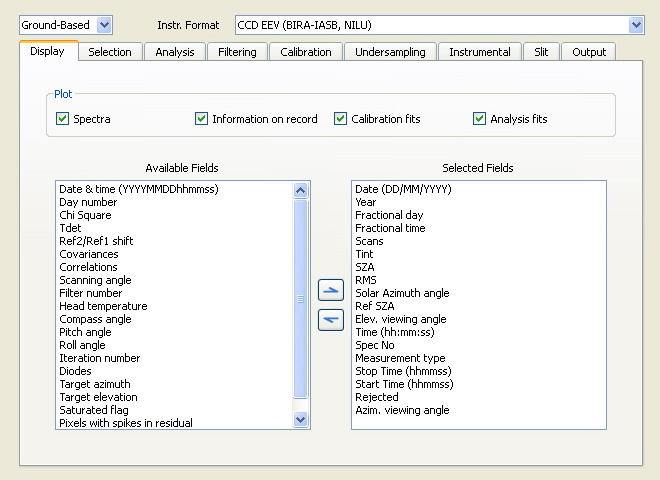
\includegraphics[width=\textwidth]{img/Project_Display.jpg}
\caption{Projects properties: Display page}\label{projects_properties_display}
\end{figure}
\FloatBarrier

The analysis of spectra can be performed in a non-stop way. Disabling the plot of spectra and fits during the analysis makes the processing significatively
faster although the use of the command line tool \textbf{doas\_cl} is recommended in this case. If the
\textbf{Spectra} button is unchecked, the state of the \textbf{Data} button has no effect.  If the \textbf{Calibration fits} button is unchecked, this will disable the display
of the calibration plots whatever the state of the buttons in the \textbf{Display frame} of the \textbf{Calibration page}.

\subsubsection{Selection Of Fields To Display}
The content of this frame is similar to the one in the \textbf{Output}
page. Information related to the measurements (e.g. date and time,
viewing angles, geolocation coordinates, \dots) can be selected in
this page and will be completed with analysis results according to
buttons checked in the \textbf{Display} frame of the \textbf{Analysis
  windows properties} dialog box. The user-defined instrument or file
format determines the list of fields available for display or
output. A non-exhaustive list of fields available for ground-based and
satellite measurements is given in appendix \textbf{~\ref{cha:output}}.

\begin{figure}[!h]
\subsection{Selection Page}\label{sec:projects_selection_page}\hfill
\vspace{-0.8\baselineskip}
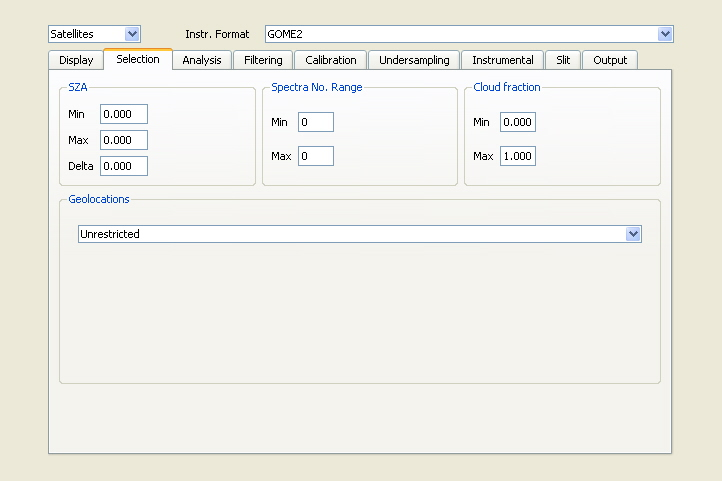
\includegraphics[width=\textwidth]{img/Project_Selection.jpg}
\caption{Projects properties: Selection page}\label{projects_properties_selection}
\end{figure}
\FloatBarrier

\subsubsection{Spectra selection}
This page is dedicated to the selection of spectra to browse or to analyse.  The selection of spectra can be made on:

\begin{longtable}[h]{l p{8cm}}
\textbf{SZA} & specify a range of solar zenith angles and a step in degrees; \\ [6pt]
\textbf{Spectra No} & specify a range of record numbers; \\ [6pt]
\textbf{Cloud fractions} & for satellite measurements, specify a range of cloud fraction (0..1). Until now, only the GOME-2 file format includes information on the cloud fraction. \\ [6pt]
\textbf{Geolocations} & for satellite measurements, selection of pixels based on the geolocation of measurements \\ [6pt]
\end{longtable}

\subsubsection{Geolocation}
Some applications just need satellite overpasses over a list of ground-based stations or above specific regions (satellite validation activities for example).  The geolocation frame gives three possibilities to select pixels over specific locations:

\begin{longtable}{l p{8cm}}
\textbf{Circle} & select pixels within a circle whose the radius is given in kilometers and whose the center could be the position of a station defined by its latitude and longitude; \\ [6pt]
\textbf{Rectangle} & select pixels above a specific region bounded by the limits in longitude and latitude given in degrees (-180..180\degree or 0..360\degree for the longitude according to the satellite file format); \\[6pt]\pagebreak % somehow, latex forgets to put a page break here
\textbf{Sites} & select pixels within multiple circles with radius given in kilometers and center position determined by the longitude and the latitude of the observation sites defined in the \textbf{Sites tab page} (see the \textbf{Output page}, page \pageref{sec:projects_output_page}, for the automatic creation of the output file name).
\end{longtable}

\subsubsection{Elevation angles}
Criteria selection on the elevation angles can be specified for MAXDOAS measurements, for example to select a reference spectrum that is not a zenith or to reject spectra measured at an elevation angle out of the specified interval.

\begin{figure}[!h]
\vspace{+0.8\baselineskip}
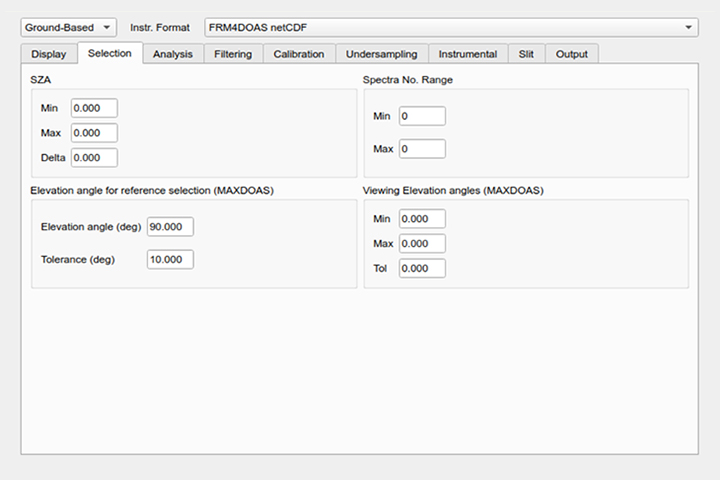
\includegraphics[width=\textwidth]{img/Project_SelectionMaxDOAS.jpg}
\caption{Projects properties: Selection page for MAXDOAS}\label{projects_properties_selection_maxdoas}
\end{figure}
\FloatBarrier

To browse or to analyse all spectra of a file without any constraint, keep default options.

\begin{figure}[!h]
\subsection{Analysis Page} \label{sec:projects_analysis_page} \hfill
\vspace{-0.8\baselineskip}
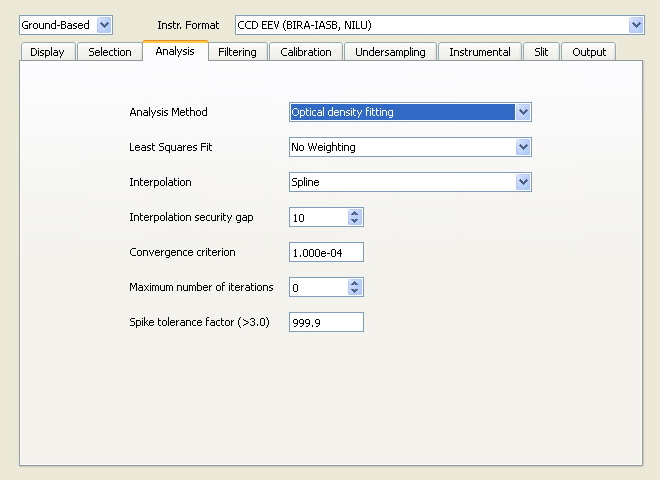
\includegraphics[width=\textwidth]{img/Project_Analysis.jpg}
\caption{Projects properties: Analysis page}\label{projects_properties_analysis}
\end{figure}
\FloatBarrier

Default options of this page are valid for all applications. Expert users can change them to perform some tests. Further details on the retrieval algorithms can be found
in the \textbf{\nameref{cha:descr-algor}} chapter.

\subsubsection{The Analysis Method}
Available retrieval method are:

\begin{itemize} \itemsep -6pt
\item Optical density fitting;
\item Intensity fitting
\end{itemize}

These methods differ by the way the Beer-Lambert equation is expressed and resolved.  Usually the \textbf{Optical density fitting} is preferred to analyze spectra.

\subsubsection{Least-Squares Fit}
The fit can be weighted if instrumental uncertainties on measurements are known.

\subsubsection{Interpolation}
\textbf{Linear} and \textbf{cubic Spline} interpolations are implemented.  \textbf{Spline} interpolation is recommended

\subsubsection{Interpolation Security Gap}
Convolution/filtering/interpolation operations could introduce edge effects if cross sections are strictly defined on the different analysis spectral intervals. In order to avoid that, it is recommended to add some extra pixels on both sides of the final grid. The security gap determines this number of pixels. If the selected filter requires a larger number of additional pixels, the gap is recalculated by QDOAS.

\subsubsection{Convergence Criterion}\label{sec:conv-crit}
As explained in the description of the \nameref{sec:marq-levenb-algor}
in section \ref{sec:doas-retrieval}, the \gls{nlls} algorithm uses the
convergence criterion to determine when it has arrived at a solution.

Usually a value of 1e-3 or 1e-4 is selected for the convergence
criterion.  For higher values of $\epsilon$, the algorithm will use
less iterations, but the accuracy of the results could be affected.

\subsubsection{Maximum Number of Iterations}
The number of iterations needed to analyze a spectrum is determined by the convergence speed of the Marquardt-Levenberg algorithm for this spectrum. For some tests, it is sometimes useful to limit it. A value of ``0'' doesn't limit the number of iterations.

\subsubsection{Spike Tolerance Factor} \label{sec:projects_analysis_spikes}
Spikes removal is a good alternative to the introduction of gaps (see the \textbf{Gaps} section of \textbf{Analysis windows properties}, page \pageref{sec:analysis_gaps_page} to automatically remove bad data points from the fit, such as
satellite measurements affected by the South Atlantic Anomaly or pixels of the detector damaged by electronic radiation.  To do this, QDOAS calculates the \gls{rms} residual after
the fit.  If a pixel $i$ is found where the absolute value of the
residual, $R_i$, exceeds the \gls{rms} by more than the spike
tolerance factor $x$,

\begin{equation}
  \label{eq:spike_removal}
  R_i > x \cdot \mathrm{RMS}\,,
\end{equation}

QDOAS will remove this pixel from the analysis and calculate a new
fit.  This procedure is applied iteratively until no residuals exceed
the \gls{rms} by more than the given tolerance factor.  The analysis results
contain a list of all pixels that were removed.

This feature should be used with caution, as choosing a too low
tolerance factor might exclude valid data points from the fit.
Assuming the residuals are normally distributed with mean 0, the
\gls{rms} can be used as an estimate of the standard deviation
$\sigma$.  As a rule of thumb, the tolerance factor $x$ should be high
enough, so the probability that a normally distributed random variable
lies outside a range of $x\cdot\sigma$ around the mean, multiplied by
the number of pixels in the analysis window, is small.

\begin{figure}[!h]
\subsection{Filtering Page} \label{sec:projects_filtering_page} \hfill
\vspace{-.8\baselineskip}
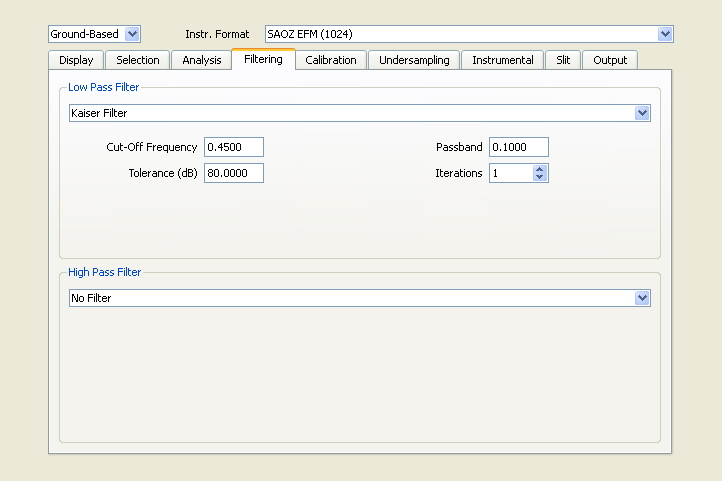
\includegraphics[width=\textwidth]{img/Project_Filtering.jpg}
\caption{Projects properties: Filtering page}\label{projects_properties_filtering}
\end{figure}
\FloatBarrier

Filtering attenuates components in the spectra with frequencies higher (low-pass filtering) or lower (high-pass filtering) than a given cut-off frequency. This simple method can improve the analysis of noisy spectra but may lead in the other hand to a loss of spectral information and should be used very carefully. Filtering corresponds to a convolution in the pixels domain.  The most common filter functions are implemented.  Further details can be found in the literature.

\begin{description}
\item[Kaiser] correction using the algorithm described in \citet{Kaiser_Reed_1977};
\item[Boxcar] convolution with a rectangle function; this filter consists in averaging the spectrum over several spectral points;
\item[Gaussian] convolution with a Gaussian function;
\item[Triangular] convolution with a triangle function;
\item[Savitzky-Golay] this filter uses a least-square linear regression fit of a polynomial of degree $k$ over at least $k+1$ data points around each point in the spectrum;
\item[Binomial] convolution with a filter function formed with the binomial coefficients calculated using the recursive Pascal's triangle algorithm;
\item[Odd-even pixels] smoothing obtained by averaging spectra interpolated on odd and even pixels.
\end{description}

According to the selected filter, different fields have to be completed.
Select filter type \textbf{No Filter} if you want to disable spectra and cross sections filtering.

Filtering is applied after interpolation of the original spectra or cross sections on the final grid.

\subsubsection{Low-Pass Filtering}
Low-pass filtering is applied to the spectra and to the cross sections. Nevertheless, the filtering of cross sections could be disabled individually in the \textbf{Analysis windows properties} dialog box.

\subsubsection{High-Pass Filtering}
Cross sections are filtered by subtracting (optical density fitting) or dividing (intensity fitting) a fitted polynomial or a smooth spectrum calculated by filtering the original cross sections a high number of times. This can be an alternative to the Gram-Schmidt algorithm to calculate differential cross sections.

For the moment, high-pass filtering is supported only in optical density fitting mode. It can be applied during the phase of calibration and/or during the analysis of spectra.

\subsection{Calibration Page}\label{sec:projects_calibration_page}
The configurtion of the wavelength calibration procedure is explained in detail in section \ref{sec:conf-wavel-calibr}.

\begin{figure}[!h]
\subsection{Undersampling Page} \label{sec:projects_undersampling_page} \hfill
\vspace{-.8\baselineskip}
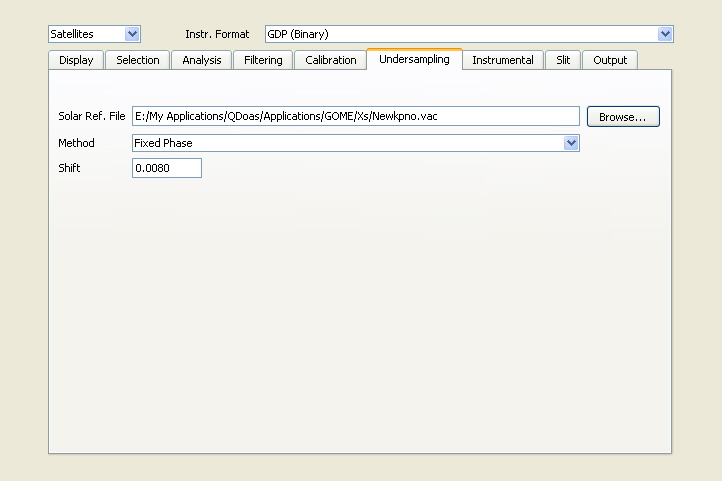
\includegraphics[width=\textwidth]{img/Project_Undersampling.jpg}
\caption{Projects properties: Undersampling page}\label{projects_properties_undersampling}
\end{figure}
\FloatBarrier

The undersampling is a well-known problem of GOME onboard the
satellite ERS-2. It arises from the poor sampling ratio of the GOME
instrument (2 to 3 pixels/\gls{fwhm} of the resolution of the
spectrometer) which results in a lost of spectral information when
interpolating earthshine spectra during the DOAS fitting process. The
problem can be corrected using ad-hoc cross sections obtained by
simulating the effect from a high-resolution solar
reference. Undersampling cross sections can be pre-calculated using
the \textbf{\nameref{sec:tool_undersampling}} or they can be
calculated in real time, just after the wavelength calibration
procedure using the corrected grid and the determined slit function.

To apply undersampling correction, the fit button of \textbf{Usamp 1} and/or \mbox{\textbf{Usamp 2}} items in the \textbf{Predefined parameters} page of \textbf{Analysis windows properties} (cfr page \pageref{sec:undersampling_params}) has to be checked in addition of the selection of options of this page.
By default, no undersampling correction is applied.

\subsubsection{Method}
Different methods for the calculation of the undersampling correction are available.
\begin{longtable}[h]{l p{8cm}}
\textbf{From file} & Undersampling cross sections are provided in files like usual cross sections. These files might be created using the \textbf{\nameref{sec:tool_undersampling}}. The files have to be provided in the \textbf{Analysis windows properties} (\textbf{Molecules} or \textbf{Predefined paremeters} page according to the selected analysis method). \\ [6pt]
\textbf{Fixed phase} & QDOAS uses the information derived from the calibration procedure to create the undersampling cross sections, with a fixed value of the shift. The selection of this method is recommended. \\ [6pt]
\textbf{Automatic phase} & The undersampling cross sections are calculated at each iteration of the analysis procedure, using the fitted value for the shift between the reference and the measured spectra. This method is rather time consuming and only applicable for testing purposes.	 \\ [6pt]
\end{longtable}

\subsubsection{Solar ref. file}
In \textbf{Fixed phase} and \textbf{Automatic phase}, undersampling cross sections are calculated from a high resolution solar spectrum convolved on an oversampled and an undersampled grid with the instrument slit function (according to \textbf{calibration options}, the slit function characterized by the calibration procedure or a slit function provided by the user in the \textbf{slit page} of \textbf{Projects properties}).

\subsubsection{Shift}
The \textbf{Shift} field operates only in \textbf{Fixed phase} method.

\begin{figure}[!ht]
\subsection{Instrumental Page} \label{sec:projects_instrumental_page} \hfill
\vspace{-.8\baselineskip}
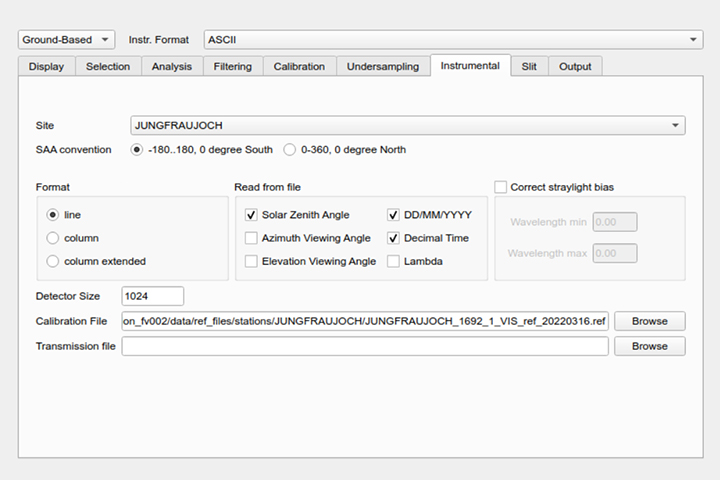
\includegraphics[width=\textwidth]{img/Project_InstrumentalAscii.jpg}
\caption{Projects properties: Instrumental page}\label{projects_properties_instrumental}
\end{figure}
\FloatBarrier

The fields that appear in this page strictly depend on the format of spectra files to process.

\subsubsection{Ground-based measurements}The size of the detector is the first information to provide in this page.  Except if a preliminary wavelength calibration is provided with the spectra, a wavelength calibration file is necessary to browse spectra.
For ground-based measurements, the observation site allows (re)calculating solar angles.  The calculated solar azimuth angles will follow the provided SAA convention.

\textbf{Important note} : Even if the native MFC binary and standard formats generated by DOASIS and MS-DOAS acquisition S/W can still be selected, no further development and support is provided.

\subsubsection{Calibration File And Instrumental Corrections}

\textbf{For the analysis of spectra, the wavelength calibration of the reference spectrum always has the priority over the spectra ones.  It is important to select this file very carefully mainly when browsing spectra to save a new reference spectrum.}

Some instrumental corrections can be applied on spectra. For example, a transmission function previously determined in laboratory with calibrated sources can be specified in the \textbf{Transmission file} field. A two columns ASCII file is expected (wavelength calibration and transmission function) and spectra will be divided by this curve before the wavelength calibration procedure.

Dark current correction is also possible according to the file format. The selected file format determines how dark currents are provided and how spectra are corrected.  See below for \textbf{Dark Current And Offset Correction for the MFC format (original binary and std formats generated by DOASIS or the one specific at BIRA-IASB}.

For satellite measurements, the wavelength calibration of earthshine spectra and irradiances is provided in the files and no transmission file is needed. Both fields should then be kept empty. The only information to provide should be the spectral region to process: the band type (for GOME and GOME2) or the channel and the clusters (for SCIAMACHY).

\subsubsection{Dark Current And Offset Correction For The MFC Format}
According to the file format, measured dark current are available and
subtracted from spectra just before the analysis.  Since version
2.111, QDOAS supports both MFC binary and STD ASCII formats generated
by the well-known DOASIS program created by the atmospheric research
group at IUP Heidelberg, Germany and widely used in the DOAS community.

\begin{center}
\href{https://doasis.iup.uni-heidelberg.de/bugtracker/projects/doasis/}{https://doasis.iup.uni-heidelberg.de/bugtracker/projects/doasis/}
\end{center}

In addition, BIRA-IASB has developed its own binary MFC format in which all spectra including dark currents and offsets of a same day are saved in a unique file.  A MFC STD to MFC BIRA-IASB binary format converter exists (see the \textbf{MFC Binary section}, page \pageref{sec:MFC_bin}).

For the BIRA-IASB binary format, dark currents and offsets present in a file are averaged before spectra correction.  For the MFC binary and std formats generated by DOASIS, dark current and offset are provided in two separate files in the original format.  Dark currents should be spectra measured with a large integration time (typically 30 sec) and offsets should be the average of a large number of spectra measured with a very small integration time (typically 1000 x 3 ms).

Application of the offset correction:
\begin{equation}
\mathrm{spe}^\prime=\mathrm{spe}-\mathrm{offset}\cdot(\mathrm{scans}_\mathrm{spe}/\mathrm{scans}_\mathrm{offset})\, ,
\end{equation}
\begin{equation}
\mathrm{drk}^\prime=\mathrm{drk}-\mathrm{offset}\cdot(\mathrm{scans}_\mathrm{drk}/\mathrm{scans}_\mathrm{offset})\, ,
\end{equation}
where $\mathrm{scans}_\mathrm{spe}$, $\mathrm{scans}_\mathrm{drk}$ and $\mathrm{scans}_\mathrm{offset}$ are respectively the number of scans for the spectrum, the dark current and the offset.

Correction of spectra with the dark current (previously corrected by offset):
\begin{equation}
\mathrm{spe}^\prime=\mathrm{spe} - \mathrm{drk}\cdot (\mathrm{et}_\mathrm{spe}\cdot\mathrm{scans}_\mathrm{spe}) /(\mathrm{et}_\mathrm{drk}\cdot\mathrm{scans}_\mathrm{drk})\, ,
\end{equation}
where $\mathrm{et}_\mathrm{spe}$ and $\mathrm{et}_\mathrm{drk}$ are respectively the exposure time of the spectrum and the dark current and $\mathrm{scans}_\mathrm{drk}$ is the number of scans of the dark current.

\subsubsection{The Observation Site}
The information on the observation \textbf{Site} is used to (re)calculate solar zenith angle from geolocation coordinates given for this site in the \textbf{Sites} sheet. This can be useful for example if the solar zenith angles saved in the files are not reliable enough. The abbreviation of the observation site is also used to automatically generate output file names (see the \textbf{Output Page}, page \pageref{sec:projects_output_page}).  The longitude is particularly useful to select reference spectra of the day using the local time instead of Universal Time in case fractional days and times given in UT are distributed in two days (for example, measurements in China).

\subsubsection{Straylight bias}
Requested for some spectra files format, this option allows subtracting from a spectrum the signal averaged on the specified range of wavelengths.
This is useful for example, to retrieve \SO2 in the UV region where the signal is very poor and where the straylight is problematic.  Even if the straylight can be attenuated by subtracting from the spectra, the average of the signal measured in the UV region (below 300 nm if possible), it is recommended to characterize it in laboratory.

\subsubsection{OMI Options}
QDOAS provides some specific options to handle OMI files.  To make
optimal use of these options, refer to the detailed description of the
OMI L1B data in the \citet{OMI_iods}.
\begin{figure}[!ht]
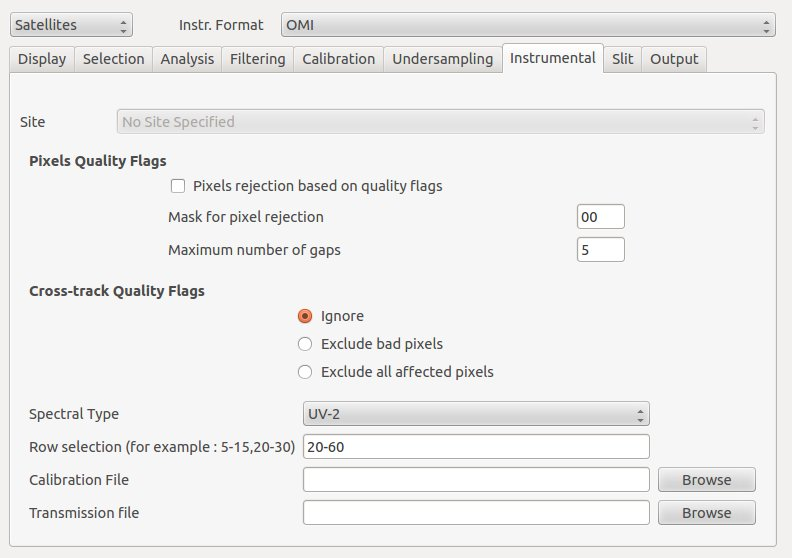
\includegraphics[width=\textwidth]{img/Project_Instrumental_OMI.jpg}
\caption{Projects properties: Instrumental page for OMI.}\label{img:project_instrumental_omi}
\end{figure}

\begin{description}
\item[Pixel Quality Flags] These flags indicate if a wavelength pixel
  was affected by measurement problems such as dark current, stray
  light or saturation.  Using this setting, QDOAS can exclude single
  pixels from the fitting procedure if certain flags are set.

  To use the flags, check ``Pixel rejection based on quality flags''.

  The field ``Mask for pixel rejection'' should contain a hexadecimal
  number indicating which flags should lead to rejection.  For
  example, to exclude pixels with flags 0, 1 and 3 set, one would
  choose a mask
  \begin{equation*}
    2^0 + 2^1 + 2^3 = 11 = \mathrm{B}_{16}\,.
  \end{equation*}
  to reject all flags, one would choose the mask
  \begin{equation*}
    2^0 + 2^1 + \ldots + 2^{15} = 65535 = \mathrm{FFFF}_{16}
    \,.
  \end{equation*}
  For a full description of the 16 PixelQualityFlags in the OMI L1B data,
  refer to the \citet{OMI_iods}.

  The value ``Maximum number of gaps'' indicates the maximum number of
  pixels that should be excluded from the spectrum.
\item[Cross-track Quality Flags] Cross-track Quality Flags describe
  the so-called ``row anomaly'' affecting the OMI data.  These flags
  apply to a complete spectrum and indicate how badly the spectrum is
  affected.  QDOAS provides three options for the handling of these
  flags (see \citep{OMI_iods}):
  \begin{description}
    \item[Ignore] Use all spectra, disregarding the quality flags.
    \item[Exclude bad pixels] Only exclude rows flagged as 'Affected,
      Not corrected, do not use' in the L1B data.
    \item[Exclude all affected pixels] Only use rows flagged as 'Not
      affected'.
  \end{description}
\item[Spectral Type] OMI measurements contain data from three spectral
  bands: UV-1, UV-2 and VIS.
\item[Row selection] This option allows the user to select a subset of
  the 60 detector rows for the analysis, by providing a list of ranges
  from 1 to 60.
\end{description}

\begin{figure}[!h]
\subsection{Slit Page} \label{sec:projects_slit_page} \hfill
\vspace{-.8\baselineskip}
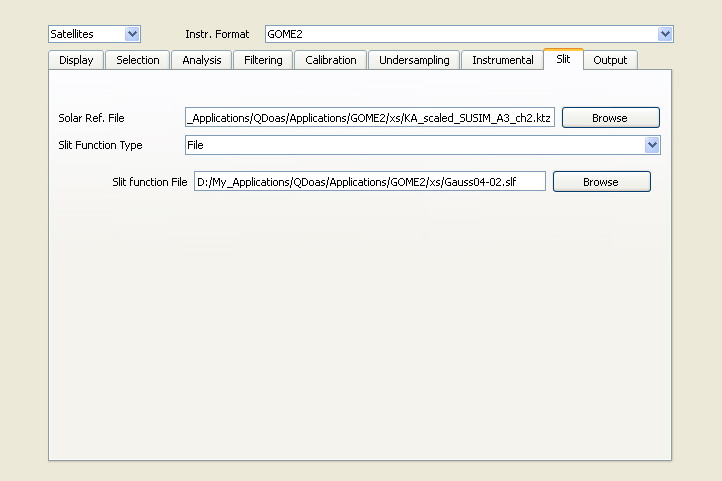
\includegraphics[width=\textwidth]{img/Project_Slit.jpg}
\caption{Projects properties: Slit page}\label{projects_properties_slit}
\end{figure}
\FloatBarrier

Input cross sections have to be degraded to the resolution of the instrument before the analysis. This can be done using the \textbf{convolution tool}. However the programme also authorizes the direct use of high-resolution cross sections which will be convolved in real time using information provided in this page \underline{\textbf{if and only if}} the slit function is not characterized by the \textbf{wavelength calibration procedure}.

\subsubsection{Slit Function Type}
Several analytic line shapes are proposed including line shapes supported by the \textbf{wavelength calibration procedure} (gaussian, lorentzian, error function, voigt and asymmetric line shapes). Different fields have to be completed according to the selected slit function. ASCII file is requested for slit functions measured in laboratory (option \textbf{File}) or when the ``Wavelength dependent'' button is checked (analytical line shapes).

\begin{itemize}
\item \underline{Slit functions measured in laboratory}: the first column should be the wavelength grid of the line shape; the maximum of the line shape is expected around 0 nm;  look-up tables can be specified for line shapes defined at different wavelengths (in this case, the first line gives the individual wavelengths).
\item \underline{Wavelength dependent analytical slit functions}: the input file should contain the \gls{fwhm} variation with the wavelenth calibration; at a given wavelength, cross sections will be convolved with the appropriate resolution.
\item \underline{Wavelength dependent stretch factors on a user-defined slit function}:
To account for an asymmetry of the slit function that varies with the wavelength, a three columns ASCII file can be specified in addition to the slit function file.  This ``Stretch on wavelength'' file should contain the wavelength calibration and the two values of the stretch to apply on the grid of the line shape, one for each side of the slit function.
Such a file can be obtained by merging in one file the parameters SFP1 and SFP2 resulting of the wavelength calibration (use the \textbf{Save As} option from the title of the plots to save the curves in an ASCII file).
\end{itemize}

\subsubsection{Solar Reference File}
A high-resolution solar spectrum is expected to replace the solar spectrum of the \textbf{Calibration page} if the slit function is not characterized during the calibration procedure and solar spectrum and cross sections have to be convolved with the line shape specified in this page.
Otherwise, if the slit function type of this page is \textbf{None}, preconvolved solar spectrum (in this page) and cross sections (in \textbf{Analysis windows properties}) are expected.

\begin{figure}[!h]
\subsection{Output Page} \label{sec:projects_output_page} \hfill
\vspace{-.8\baselineskip}
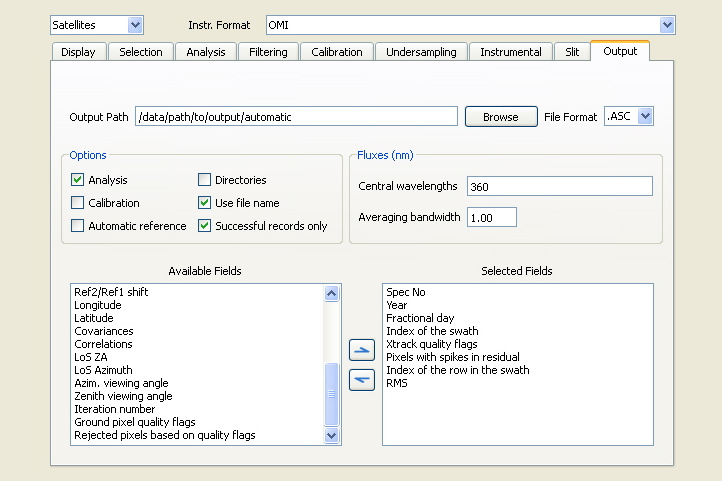
\includegraphics[width=\textwidth]{img/Project_Output.jpg}
\caption{Projects properties: Output page}\label{projects_properties_output}
\end{figure}
\FloatBarrier

This page is dedicated to the selection of information on analyzed records to write in the output file after calibration and/or analysis of spectra. When the \textbf{Analysis button} is checked, all the fields in this page are enabled and it is also possible to select the fit results that should be saved in the \textbf{Analysis windows properties} pages.

When the user selects chooses ``.ASC'' as the file format, the program produces ASCII files with tab-separated columns for all selected output fields.  These files may be loaded in spreadsheets such as Excel.  The first line of the analysis output starts with a hash (\#) character and is used to print the column titles.  When the \textbf{Calibration button} is checked, wavelength calibration results are saved before the analysis results. Lines with calibration output start with a semicolon (;).  \textbf{If an ASCII output file already exists at the specified location, QDOAS appends the new results to the existing file.}  In this case, column titles and calibration information are not repeated.  Therefore, it is best to avoid writing to existing files, unless exactly the same analysis and output configuration is used to produce the new data.  \textbf{To replace the content of an existing output file, the file must first be deleted manually}.

With the file format ``.nc'', QDOAS will produce netCDF output data.
This is the recommended setting for users who wish to use a binary
output format.  In contrast to ASCII mode, results from different
processing runs cannot be appended to the same file in netCDF mode,
unless the user chooses a different group name for both runs (the
default group name is the project name).  When using QDOAS with a
single output file, the program will check if a netCDF file with that
filename already exists, and report an error if the file already contains a group with the chosen group name.  However, when writing files in ``automatic'' mode
(see \nameref{sec:autom-creat-outp}), QDOAS doesn't check in advance
which output file(-s) it will have to write, and it is left to the
user to make sure that there are no existing files in the output path
which will prevent QDOAS from saving the results of a processing run.

QDOAS always saves all the output from a single input file in one shot, either when it has processed the last spectrum of an input file, or when the analysis is stopped using the \textbf{stop button} 
\includegraphics[width=3mm]{img/Button_Stop.png}.

By default, QDOAS only saves records successfully analyzed.  If the button \textbf{Successful records only} is kept unchecked, all records including reference spectra and records for which the analysis fails (e.g. log error on the spectrum) are saved.

When processing was unsuccessful, QDOAS uses the fill value
9.969\ldots e+36 for floating point output data, an empty string for
text output fields, and values -32767, 65535 or -2147483647 for
integer output fields, depending on the range of the output field.
For the netCDF output format, fill values are written to the
\_FillValue attribute of the corresponding variables.

\subsubsection{Automatic Creation Of The Output File Name}\label{sec:autom-creat-outp}
The path and the name of the output file can be specified in the \textbf{Output Path} field.  If ``automatic'' is used as a file name, QDOAS will generate the name of the output file automatically, using the user-defined output path as a base.

For ground-based measurements, the \textbf{Directories} and \textbf{Automatic reference} buttons have no effect. The original file name is always used (but the file extension is changed in \textbf{``.asc''}) except if the \textbf{Use file name} button is unchecked and an observation site has been specified in the \textbf{Instrumental page}. In this case, the output file name is built as follows:
\begin{center}
$<$output path$>$/XXYYYYMM.ASC
\end{center}
Where:

\begin{longtable}[h]{l p{8cm}}
\textbf{output path} & is the user-defined path; \\ [6pt]
\textbf{XX} & is the abbreviation of the observation site selected in the \textbf{Instrumental} tab page; if no observation site is specified, the original file name is used; \\ [6pt]
\textbf{YYYY} & is the year of measurement; \\ [6pt]
\textbf{MM} & is the month (zeros padded) of measurement; \\ [6pt]
\textbf{ASC} & is the default file extension for ASCII files;	\\ [6pt]
\end{longtable}

For satellite measurements, the \textbf{Use file name} button has no effect. If overpasses calculation is requested (option \textbf{Sites} in the \textbf{Geolocation} frame of the \textbf{Selection} page), then the output file name is determined as above ($<$output path$>$/XXYYYYMM.ASC where XX is the abbreviation of the station). Otherwise, for SCIAMACHY files, the output file name automatically created has the syntax SCIA\_YYYYMMDD\_NNNN.ASC where YYYYMMDD is the date of measurement (year, month, day) and NNNN the orbit number. For other satellite formats, the original file name is used (but with the file extension \textbf{``.ASC''}). Files are distributed in a year/month/day folder structure if the \textbf{Directories} button is checked.

\subsubsection{Fluxes}
The \textbf{flux} is the value of the signal averaged over pixels within a bandwith around the specified wavelength.  Divided by the exposure time, this can be used to check a relative intensity.  To calculate and save fluxes in the output file, specify the central wavelengths separated by the semicolon (;) character. For example, to get fluxes at 330 nm, 350 nm and 380 nm, enter:
\begin{center}
330; 350; 380;
\end{center}
The averaging bandwidth in nm is also requested (for example a bandwidth of 1 nm means that pixels within the central wavelength +/- 0.5 nm will be averaged).
Coulour indexes are the ratio between two fluxes and can be easily recalculate from output fluxes.

\subsubsection{Selection Of Fields To Output}
The content of this frame is similar to the one in the \textbf{Display page}.  In QDOAS, the output is fully configurable. Information related to the measurements (e.g. date and time, viewing angles, geolocation coordinates,~\dots) can be selected in this page. The selection of analysis results (e.g. slant column densities, fitted non-linear parameters,~\dots) is made individually in the \textbf{Analysis windows properties} pages. The selected instrument or file format determines the list of fields available for output. For example, information on cloud fraction and cloud top pressure is available only for satellite instruments. A non-exhaustive list of fields available for ground-based and satellite measurements is given in appendix \textbf{\ref{cha:output}}.

\begin{figure}[!h]
\section{Analysis windows properties}
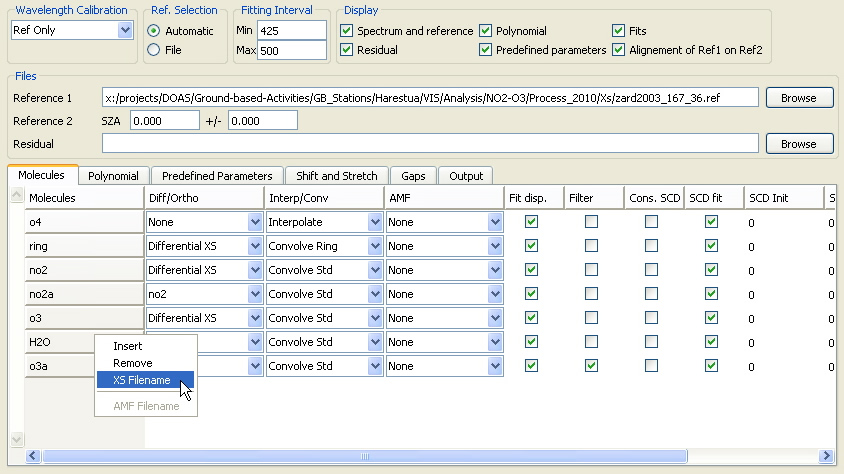
\includegraphics[width=\textwidth]{img/Analysis_Properties.jpg}
\caption{Analysis windows properties}\label{analysis_properties}
\end{figure}
\FloatBarrier

This dialog box completes the \underline{\textbf{Projects properties}} for the configuration of the analysis of spectra. Several analysis windows can be defined under a same project.  Next section will guide you in the definition of parameters to fit.

\subsubsection{Fitting interval}
The fitting interval is the first option to specify when a new analysis window is created. It depends on the region covered by the spectrometer and the trace gases to retrieve. According to the molecules to focus on, some baseline recommendations can be found in the literature.

\subsubsection{Reference Spectra}
In the DOAS technique, spectra are always analyzed with respect to a reference spectrum. This could be the irradiance spectrum of the current satellite file, any other reference spectrum provided in an ASCII file or a daily reference spectrum selected on a solar zenith angle criterion. The \textbf{Ref. Selection} box proposes to choose between the modes \textbf{File} (irradiance of the file for satellites measurements or an external reference spectrum) and \textbf{Automatic} (reference spectrum selected on specific criteria).

In addition, QDOAS gives the possibility to define two reference spectra (\textbf{Reference 1} and \textbf{Reference 2}). \textbf{Reference 1} is always a file; according to the \textbf{Ref. Selection mode}, \textbf{Reference 2} can be the name of an ASCII file or a spectrum automatically selected by the program. These options determines on which reference spectrum the wavelength calibration procedure is applied:
\begin{itemize}
\item If only one reference spectrum is specified (\textbf{Reference 1} or \textbf{Reference 2}), it is used as control spectrum i.e. the \I0 spectrum in the Beer-Lambert law. The wavelength calibration procedure is applied on this spectrum and the cross sections are re-interpolated on the new calculated grid before the analysis of spectra.
\item If two reference spectra are given, the wavelength calibration is applied only on the first one (\textbf{Reference 1}); the shift between both reference spectra is then determined (using a \gls{nlls} fitting approach) in order to align cross sections on the second reference spectrum (\textbf{Reference 2}) and spectra are analysed w.r.t. \textbf{Reference 2}.
\end{itemize}

\subsubsection{Automatic Reference Selection}
The information on the \gls{sza} is present in most ground-based file formats.  According to the SZA range, a reference spectrum with the SZA the closest to the given value is selected for each twilight or the spectrum with the minimum SZA of the day is selected (both values initialized to 0 or the SZA range below all SZA values of the file).

For \textbf{MAXDOAS measurements}, it is also possible to select the zenith spectrum of the scan.  Currently, \textbf{Scans/SZA} radio buttons appear to make this selection possible with the BIRA-IASB CCD EEV format, MFC binary and std formats generated by DOASIS, MFC BIRA binary format and ASCII format.  If this option is necessary for other file formats, please, contact \href{mailto:caroline.fayt@aeronomie.be}{authors}.

\begin{figure}[!h]
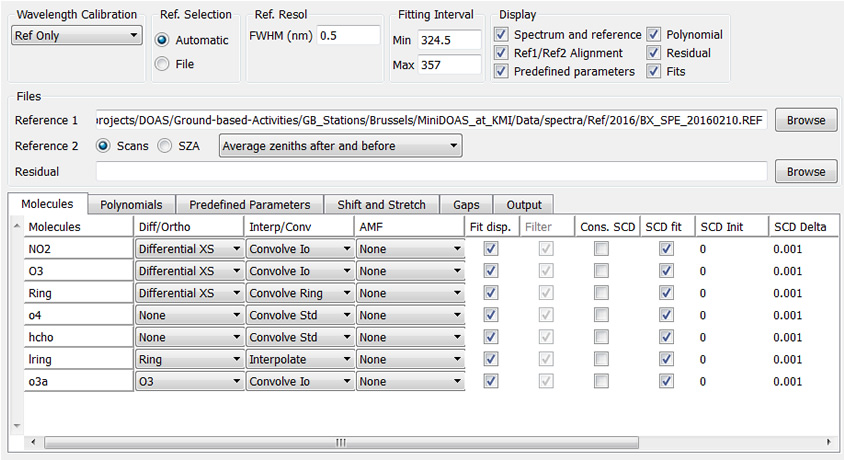
\includegraphics[width=\textwidth]{img/Analysis_Properties_Scans.jpg}
\caption{Automatic reference selection in scan mode for MAXDOAS measurements}\label{analysis_properties_scans}
\end{figure}
\FloatBarrier

Currently, in mode ``reference of the scan'', four options are available :

\begin{itemize} \itemsep -3pt
\item select the last zenith before the current scan;
\item select the first zenith after the current scan;
\item average the zenith spectra before and after the scan;
\item interpolate at the current measurement time, the zenith spectra before and after the scan.
\end{itemize}

Note that if one of the two zenith spectra (the zenith just before or after the current scan) is missing, the other one is automatically used as reference.

For \textbf{satellite measurements}, if no \textbf{Reference 1} is specified (field kept empty), the irradiance of the current file is always implicitly used. This means that if a \textbf{Reference 2} is provided, the wavelength calibration is applied on the irradiance spectrum (\textbf{Reference 1}) of the file and the control spectrum (\textbf{Reference 2}) will be aligned on the irradiance before the analysis of earthshine spectra.  For satellite measurements, the \textbf{Reference 2} spectrum could be an average of spectra selected in a specific region given by its minimum and maximum latitudes and longitudes. Other information such as the cloud fraction (GOME2) could also be used to refine the reference selection.
% TODO detailed info on automatic reference selection procedure for OMI/GOME2/other satellite instruments?

\subsubsection{Wavelength Calibration}
The quality of the fit results largely relies on a very accurate determination of the wavelength calibration of the reference spectrum.  The wavelength calibration procedure developed in QDOAS allows correcting the preliminary grid of the reference spectrum using a high-resolution solar atlas spectrum degraded to the resolution of the instrument (see the \textbf{Calibration page}, page \pageref{sec:projects_calibration_page} of \textbf{Projects properties}).  The information on the shift and eventually the slit function retrieved from this procedure are used to convolve/interpolate the cross sections before the analysis.  The wavelength calibration is always applied in priority on the \textbf{Reference 1} (the irradiance spectrum for satellite measurements). If two reference spectra are provided, \textbf{Reference 2} is aligned on \textbf{Reference 1} using the same non linear least-square algorithm as the one used for the analysis of spectra w.r.t. the control spectrum.

If the wavelength calibration of the reference spectrum is assumed to be accurate enough, the option \textbf{None} can be used instead of \textbf{Ref Only}. The option \textbf{Spectra only} is useful for some particular applications (for example, long paths measurements for which the reference spectrum is a lamp measurement).

The option \textbf{Ref+spectra} allows applying a calibration correction on both reference spectrum and spectra to analyze. This option has been designed to handle spectra recorded with unstable (unthermostated) instruments where the spectral resolution can vary a lot from one spectrum to another. In this case, the resolutions of both spectra are matched to the resolution of the less resolved spectrum, and the absorption cross sections can be convolved in real-time to the same effective resolution. This option is time consuming and should be used carefully.

\subsubsection{Display}
After the processing of a spectrum, QDOAS can plot for each spectral analysis window:
\begin{itemize} \itemsep -3pt
\item the spectrum and the reference in the fitting interval;
\item the residual of the fit (the difference between the observed and the calculated);
\item the continuum part of the spectrum fitted by a polynomial;
\item the fit obtained for each species
\item the predefined parameters (offset, undersampling);
\item in the case two reference spectra have been selected, these two spectra after the alignment correction.
\end{itemize}
The appropriate buttons are checked according to the graphs to plot.  An individual selection of the cross sections and the predefined parameters can still be performed in the dedicated tab pages.

\subsubsection{Residuals}
If a file is specified in the \textbf{``Residual''} filename field,
Qdoas will use this file to output the fitting residuals.  This
feature can be used in order to study the residuals, or, when
systematic residual structures structures are identified, in order to
create a synthetic cross section that could be introduced in the fit.
Because Qdoas appends the residuals of each analysis run to the end of
the file, the size of the file can increase rapidly and it is
recommended to disable this option by emptying the
\textbf{``Residual''} file name field when it is no longer needed.

The residual file contains one line for each processed record.  The
first three numbers are the record number, the solar zenith angle and
the decimal time respectively.  Then, the residuals for each wavelength
of the original spectrum are given.  For wavelengths which are not
part of the chosen analysis window, or which were removed by the spike
removal algorithm, a ``nan'' value is written.  The first line of the
file contains the calibrated wavelength for each column, preceded by
the three numbers \texttt{0 0 0}.  An example:

\begin{Verbatim}[fontfamily=courier,fontsize=\relsize{-2}]
0 0 0 4.25848e+002 4.25689e+002...  4.99708e+002 5.00065e+002
16 81.024 7.2989 nan ... nan -3.992e-004 ...  -6.663e-005 2.460e-004 nan ... nan
17 80.668 7.3006 nan ... nan 3.584e-004 ...  1.611e-004 9.982e-004 nan ... nan
18 80.396 7.3019 nan ... nan 2.594e-004 ...  7.704e-005 9.206e-004 nan ... nan
\end{Verbatim}

\subsubsection{Fitting Parameters}
The user must define the fitting parameters in the appropriate pages of the property sheet at the bottom of the dialog box. The different pages are:

\begin{description}
\item[Molecules] definition and configuration of the list of cross sections to fit;
\item[Polynomials] specification of the degree of the polynomial used to fit the continuous component of the absorbance, and the polynomial used for linear offset fitting;
\item[Predefined Parameters] this page proposes several predefined parameters such as offset, undersampling, \dots  ;
\item[Shift and Stretch] shift and stretch can be applied to any spectral item;
\item[Gaps] gaps can be introduced in the fitting window (e.g. to eliminate bad pixels)
\item[Output] selection of the calculated column densities and associated errors that should saved in the output file.
\end{description}

According to the associated type of parameters, the selected page proposes several columns of options to fill in, to check or to select from a multiple choice. The conviviality of the analysis parameterisation is enhanced by the use of right-click shortcut menus to handle the lists of items in the different tab pages.  Because of the complexity of the whole set of options, the structure is detailed page after page in the following section.

\section{Configuration of the fitting parameters} \label{sec:analysis_config_param}
\subsection{The Molecules Page}
This page contains options for defining and configuring the list of cross sections to fit (see figures below):

\begin{figure}[!h]
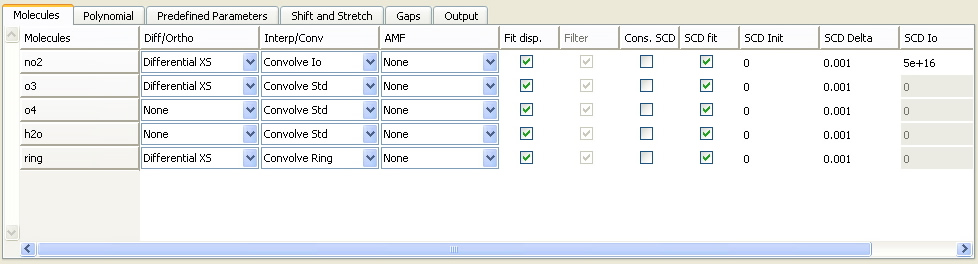
\includegraphics[width=\textwidth]{img/Analysis_Molecules.jpg}
\caption{Analysis Windows Properties: Molecules Page}\label{analysis_molecules}
\end{figure}
\FloatBarrier

Molecules are characterized by their cross section. They are represented by symbols previously defined in the \textbf{Symbols} page of the user interface. QDOAS needs these symbols for internal use: to create lists of available molecules for specific options (for example: in the \textbf{Differential cross sections} column or in the \textbf{Shift and stretch} page) and to build cross section files filters.
\begin{itemize}
\item \textbf{For internal needs of the program, cross section files names must imperatively start with the symbol name as prefix followed by the underscore character !}
\item There is no constraint on the cross section file extension; the default one used by QDOAS for creating cross sections files filters starts with ``xs''.
\end{itemize}
Right-click and select \textbf{Insert}, \textbf{Remove} or \textbf{XS Filename} options in the contextual menu respectively to insert a new molecule in the list, to delete an existing one or to modify the file associated to a cross section. The \textbf{Remove} option is disabled for a symbol if another cross section is orthogonalised to the selected one or if the selected symbol is used in the \textbf{Shift and Stretch} pages.

\subsubsection{Differential cross sections} \label{differential_xs}
Differential cross sections can be generated by orthogonalisation or high-pass filtering according to the definition of an orthogonal base formed with the component vectors (generally, a base of order 2) of the polynomial defined in the \textbf{Polynomial} page. Refer to the \textbf{\nameref{cha:descr-algor}} chapter for further details.  Three options are available:

\begin{description}
\item[None] the original cross section is used;
\item[Differential XS] a differential cross section is generated, either
  \begin{enumerate}
  \item by orthogonalisation if an orthogonal base is defined in the \textbf{Polynomial} page (Gram-Schmitt algorithm);
  \item using high-pass filtering options defined in the \textbf{Filter} tab page of \textbf{Projects properties} otherwise.
  \end{enumerate}
\item[Cross section] When choosing another cross section from the
  proposed list, the selected cross section is orthogonalised to the
  orthogonal base (if defined) and to the cross section chosen from
  the list (orthogonalisation in cascade is allowed).
\end{description}

The latter case prevents from possible correlation between two cross sections (for example, two \ozone~cross sections measured at different temperatures typically to separate contributions from the stratosphere and the troposphere or cross sections with strongly correlated absorption structures, eg. \BrO~and \H2CO). The list of available cross sections includes all cross section symbols defined in this page except the one selected. It is updated as cross sections symbols are added to or removed from this page.

\subsubsection{Interpolation/Convolution}
Cross sections should be defined on the grid of the control spectrum before the analysis. This column describes the action to perform on the selected cross section:

\begin{longtable}[h]{l p{8cm}}
\textbf{None} & the selected cross section is assumed to be correctly aligned on the reference spectrum grid; so, no action will be performed on the cross section (for example, a user-defined undersampling cross section in optical density fitting); \\ [6pt]
\textbf{Interpolate} & the selected cross section will be interpolated on the grid of the reference spectrum; a cross section already pre-convolved at the resolution of the instrument is expected in input. \\ [6pt]
\textbf{Convolve Std} & this option gives the possibility to convolve a high-resoluted cross section in real-time using either the information on the calibration and the slit function provided by the \textbf{wavelength calibration procedure} or the user-defined slit function specified in the \textbf{Slit Function page} of \textbf{Projects properties}. If the wavelength calibration procedure is applied on both the control spectrum and spectra to analyse, the cross section is convolved with the poorest resolution; \\ [6pt]
\textbf{Convolve \I0} & the cross section is convolved with \I0 correction using the concentration defined in the column \textbf{$SCD$ \I0} (this is the slant column density of the cross section used to calculate the theoretical optical depth in convolution with \I0 correction (see \citet{aliwell_2002}); \\ [6pt]
\textbf{Convolve Ring} &	in the same way, the program can generate a Ring cross section; the expected input file must be a Ring cross section pre-calculated by the \textbf{QDOAS Ring tool} on a high-resoluted grid;  \\ [6pt]
\end{longtable}

Convolving cross sections in real time is a comfortable option that avoid the pre-convolution of all cross sections with respect to the selected reference spectrum and the calibration options.

\subsubsection{AMF}
Usually, it is better to calculate vertical columns outside of QDOAS using an appropriate radiative transfer model (e.g. \glslink{lidort}{LIDORT}, \glslink{disort}{DISORT}). Nevertheless, QDOAS gives the possibility to calculate vertical columns or to correct a cross section using pre-calculated \gls{amf} through options proposed in the \textbf{AMF} column:
\vskip 6pt
\begin{longtable}[h]{p{2.5cm} p{9.cm}}
\textbf{SZA} & vertical columns are calculated using AMF depending only on the solar zenith angle; \\ [6pt]
\textbf{Climatology} & vertical columns are calculated using climatological air mass factors; the AMF depends on the solar zenith angle and the calendar day; \\ [6pt]
\textbf{Wavelength} & before the analysis, the selected cross section is corrected using wavelength dependent AMF (modified DOAS). \\ [6pt]
\end{longtable}

Additional option \textbf{AMF Filename} is proposed in the contextual menu to complete with the name of the file containing the AMF (see the requested file format according to the selected AMF option in appendix \textbf{\ref{cha:input-files-format}}).

\subsubsection{Control Of Parameters To Fit}
QDOAS minimises residuals of the DOAS equation using a Marquardt-Levenberg \gls{nlls} fitting algorithm. The method implements a gradient-expansion algorithm, which is based on the iterative combination of a steepest-descent method (suitable for approaching the minimum from far away) and a linearisation of the fitting function.

\begin{itemize}
\item In ``optical density fitting'', slant column densities of the molecules are fitted linearly and the \textbf{SCD Init}, \textbf{SCD Delta}, \textbf{SCD min} and \textbf{SCD max} buttons are ignored. Nevertheless, if the \textbf{SCD Fit} button is unchecked, the weight of the selected cross section in the optical density is fixed at the concentration value given in the \textbf{SCD Init} column.
\item In ``intensity fitting'', the slant column densities of the molecules are non linear parameters. The initial concentration value and the initial delta value used by the non-linear algorithm to calculate numerically partial derivatives of the fitting function are respectively given by \textbf{SCD Init} and \textbf{SCD Delta}. The \textbf{SCD Delta} default value shouldn't be modified except if the system seems not to converge.  \textbf{SCD min} and \textbf{SCD max} can be used to constrain the concentration of the molecules within a given interval even if it is not recommended to do that.
\end{itemize}

The selection of the analysis method is made in the \textbf{Analysis page} of \textbf{Projects properties}. Further details on the retrieval algorithms can be found in the \textbf{\nameref{cha:descr-algor}} chapter.

\underline{\textbf{For advanced users}}: it is possible to constrain the slant column density of a molecule to the value calculated in the previous analysis window.

\hspace{1cm}\parbox{11.5cm}
{
If the \textbf{Cons SCD} button is checked, the \textbf{SCD Fit} button is unchecked and the \textbf{SCD Init} value is 0., the slant column density of the selected molecule is not fitted but initialized to the value calculated in the previous analysis window if any.
}

\subsubsection{Fit display}
This column is active only if the \textbf{Fits} button is checked in the \textbf{Display} frame of the current dialog box. It allows selecting which cross sections fits will be displayed. Note that the display of the fits of all spectral analysis windows could be disabled from \textbf{Display Page} of \textbf{Projects properties}.

\subsubsection{Filter}
This column is active only if a low-pass filter has been selected in \textbf{Filtering Page} tab page of \textbf{Projects properties}. It allows defining individually which cross sections are to be filtered.

\subsection{The Polynomials Page}
The degree of the polynomial fitting the smooth component of the spectra is
specified in this page.

\begin{figure}[!h]
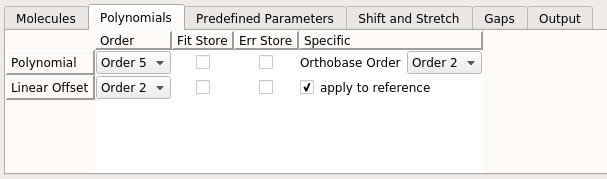
\includegraphics[width=\textwidth]{img/Analysis_Polynomials}
\caption{Analysis Windows Properties: Polynomial Page}\label{analysis_polynomial}
\end{figure}
\FloatBarrier

The values of the fitted coefficients account for the normalization
applied on both the spectrum and the reference. \textbf{Differential
  cross sections} can be generated by orthogonalisation of cross
sections w.r.t.\ an orthogonal base constructed out of the polynomial
components.  Generally, a base of order 2 is used. The
\textbf{OrthoBase} order column specifies the degree of this
orthogonal base.

To correct for instrumental and/or atmospheric straylight or residual
dark current signal, QDOAS can fit an offset parameter.  Normally,
offset is fit as a non-linear parameter, which can be configured in
the \textbf{Predefined Parameters} tab.  In some specific cases
(typically, in the near UV, around 300 nm), where the signal of the
spectrum is very low, it is better to fit offset as a linear
parameter, in order to avoid logarithm errors in when resolving the
DOAS equation (see section \ref{sec:offset-correction} for more
details).  When linear offset is enabled, a polynomial
$\mathrm{offset}(\lambda)$, normalized by the current spectrum is
included in to the DOAS fit:
\begin{equation}
\label{eq:linear_offset}
\mathrm{log}(I(\lambda))=\mathrm{log}(I_0(\lambda))-\sum{\sigma_ic_i}+\frac{\mathrm{offset}(\lambda)}{I(\lambda)}\,.
\end{equation}
The ``Order'' setting controls the order of the polynomial $\mathrm{offset}(\lambda)$.

Because the current spectrum appears in the denominator in equation
\eqref{eq:linear_offset}, QDOAS needs to solve a new linear system of
equations for every spectrum $I(\lambda)$, which can significantly
increase the processing time for a large analysis.  To work around
this, we can also apply the offset correction to the reference
spectrum, in which case the polynomial is normalized by the current
reference spectrum instead, and the fitting equation becomes
\begin{equation}
\label{eq:linear_offset_ref}
\mathrm{log}(I(\lambda))=\mathrm{log}(I_0(\lambda))-\sum{\sigma_ic_i}+\frac{\mathrm{offset}(\lambda)}{I_\mathrm{ref}(\lambda)}\,.
\end{equation}
This option can be enabled using the checkbox ``apply to reference''.

Note that a linear and a non-linear offset should not be fitted at the
same time in one spectral analysis window.

\subsection{The Predefined Parameters Pages}
This page proposes different parameters that can be fitted linearly or non linearly according to the fitting method:

\begin{itemize} \itemsep -6pt
\item scaling factor for the control spectrum (\textbf{Sol});
\item offset;
\item common residuals (\textbf{Com}).
\item undersampling (\textbf{Usamp1} and \textbf{Usamp2});
\item synthetic cross section to fit very small differences in the resolution between the spectrum and the reference (\textbf{Resol})
\end{itemize}

\begin{figure}[!h]
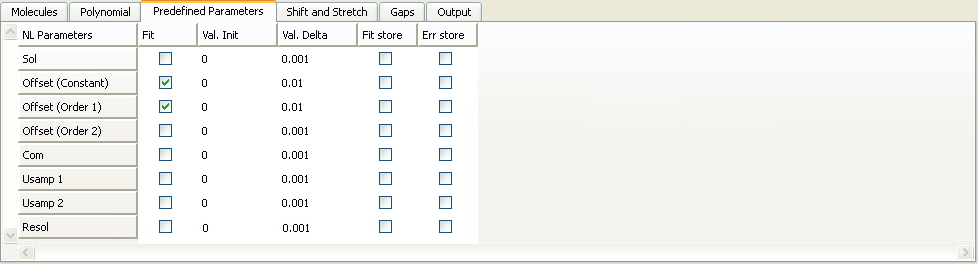
\includegraphics[width=\textwidth]{img/Analysis_Predefined.jpg}
\caption{Analysis Windows Properties: Predefined Parameters Page}\label{analysis_predefined}
\end{figure}
\FloatBarrier

A cross section file is always expected for \textbf{Com} parameter. A cross section file is expected for \textbf{Usamp1} and \textbf{Usamp2} parameters if the method \textbf{``File''} has been selected in the \textbf{Undersampling} page of \textbf{Projects properties}. To specify the name of the cross section file, right-click the \textbf{``Select~File''} option from the parameter line.

\textbf{Val init} and \textbf{Val delta} are respectively the initial value and convergence factor, two parameters used by the \gls{nlls} algorithm. In general, the default values should not be modified, except in case of convergence problems. \textbf{Fit store} and \textbf{Err store} columns are enabled only if the \textbf{Analysis button} is checked in the \textbf{Output} tab page of \textbf{Projects properties}.

\subsubsection{Offset}
An ideal spectrometer in an ideal atmosphere would measure the part of the sunlight that has been elastically scattered by air molecules and particles in the zenith direction. In a real experiment however a number of possible additional sources of signal may add up to the ideal Rayleigh/Mie contribution leading to ``offset'' the measured intensity by a certain amount. In addition to the Ring effect, which is to a first approximation a natural source of offset, instrumental sources of offset also need to be considered like stray light in the spectrometer and dark current of the detector. This is the purpose of the offset parameter which is better described in the \textbf{\nameref{cha:descr-algor}} chapter. The offset is normalized w.r.t. the intensity of the spectrum.

In some specific cases (typically, in the near UV, around 300 nm), the signal of the spectrum is very low and in order to avoid systematic logarithm errors when resolving the DOAS equation, the fit of a linearized offset is preferred (see the \textbf{Polynomial} page). Note that a linear offset and a non linear offset should not be fitted in the same spectral analysis window.

\subsubsection{Common residual}
When systematic structures appear in the residuals, it is sometimes useful to eliminate them using a synthetic cross section obtained by averaging some of such residuals (cfr the \textbf{``Residual''} field in the \textbf{Files} frame of this dialog box). In DOAS fitting, this cross section can be introduced either in the \textbf{Molecules} page with a user-defined symbol or in this page with the predefined symbol ``\textbf{Com}''. In intensity fitting, it is recommended to use the predefined symbol \textbf{Com} that is always fitted linearly whatever the analysis method.

\subsubsection{Undersampling} \label{sec:undersampling_params}
The undersampling is a well-known problem of GOME onboard the satellite ERS-2. It arises from the poor sampling ratio of the GOME instrument (2 to 3 pixels/\gls{fwhm} of the resolution of the spectrometer) which results in a lost of spectral information when interpolating earthshine spectra during the DOAS fitting process. The problem can be corrected using ad-hoc cross sections obtained by simulating the effect from a high-resolution solar reference. If the fit button of \textbf{Usamp 1} and/or \textbf{Usamp 2} items is checked, the options of the \textbf{Undersampling} page of \textbf{Project properties} (cfr page \pageref{sec:projects_undersampling_page}) are used to calculate undersampling cross sections.  In \textbf{From file} method, undersampling cross sections can be pre-calculated using the \textbf{QDOAS undersampling tool}.

\subsubsection{Resol synthetic cross section}
This cross section is built automatically by dividing the selected reference spectrum with itself but convolved with a gaussian with a FWHM of 0.05 nm.  It allows accounting for very small differences in the resolution of the reference spectrum and the spectrum to analyze.

\subsection{The Shift and Stretch Page} \label{sec:shift_stretch_page}
Shift and stretch parameters allow correcting for possible misalignment between the various spectral items involved in the data evaluation (i.e. measured and reference spectra as well as absorption cross sections). The equation below gives the wavelength transformation to apply when a shift and a stretch order 2 are fitted:

\begin{equation}
\Delta= a+b.(\lambda-\lambda_0)+c.(\lambda-\lambda_0)^2
\end{equation}

Less used, the scaling parameter consists in a wavelength dependent scaling factor to apply to a cross section. It can also be order 1 or order 2.

\begin{figure}[!h]
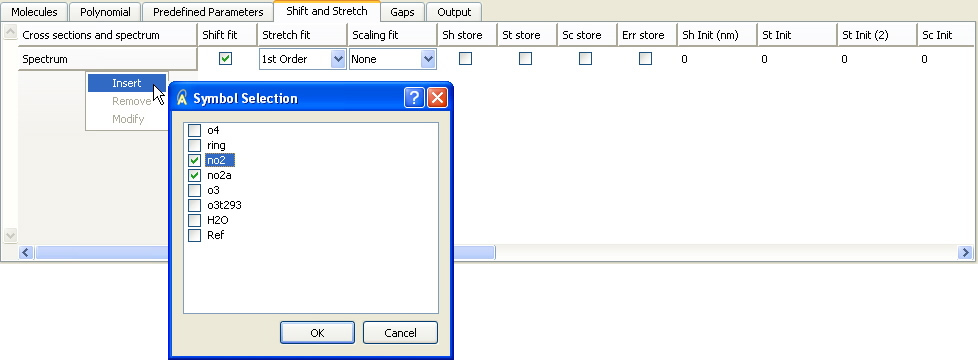
\includegraphics[width=\textwidth]{img/Analysis_Shift.jpg}
\caption{Analysis Windows Properties: Shift and Stretch Page}\label{analysis_shift}
\end{figure}
\FloatBarrier

To add an item to shift, stretch or scale, right-click the \textbf{Insert} option to open a dialog box with the list of available symbols (all cross sections defined in the \textbf{Molecules} page and completed with \textbf{Spectrum} and \textbf{Ref} symbols). It is possible to select only one or several symbols. In the latter case, the same shift and stretch parameters will be applied to all items of the selection (in the example above, the same shift and stretch will be applied on both \NO2 cross sections). After the validation of the selection, QDOAS automatically updates the list of available symbols so that a symbol can not be selected twice.

\textit{Note that a symbol can not be removed from the \textbf{Molecules} page as long as it is used in the \textbf{Shift and Stretch} page.}

\subsubsection{Output}
Buttons in the \textbf{Sh store}, \textbf{St store} and \textbf{Sc store} columns are enabled only if the \textbf{Analysis} button is checked in the \textbf{Output page} of \textbf{Projects properties}. They allow saving respectively the fitted values for the shift, the stretch and the scale. If buttons in the \textbf{Err store} column are checked, the standard deviations of the fitted parameters are also saved in the output file.

\subsubsection{Initial and delta values}
The shift, stretch and scale parameters are fitted non linearly by the Marquardt-Levenberg \gls{nlls} algorithm. This iterative method needs to start from an initial solution given by \textbf{Init} values of parameters to fit. The convergence parameters \textbf{Delta} are used by the algorithm to numerically calculate partial derivatives of the fitting function and to determine the direction of the steepest descent to approach the solution. There is one \textbf{Init} column and one \textbf{Delta} column for each parameter to fit (shift, stretch order 1, stretch order 2, scaling order 1 and scaling order 2).

\subsubsection{Convergence control}
In case of convergence problems or for safety reasons, the range of values allowed for the shift can be limited to a specified interval (\textbf{Sh Min} and \textbf{Sh Max}).

\subsection{The Gaps Page}\label{sec:analysis_gaps_page}
Gaps can be introduced in order to eliminate bad pixels from the fitting interval.  Note that using the ``Spikes removal'' feature (cfr page \pageref{sec:projects_analysis_spikes}) is a good alternative to automatically remove bad pixels.

\begin{figure}[!h]
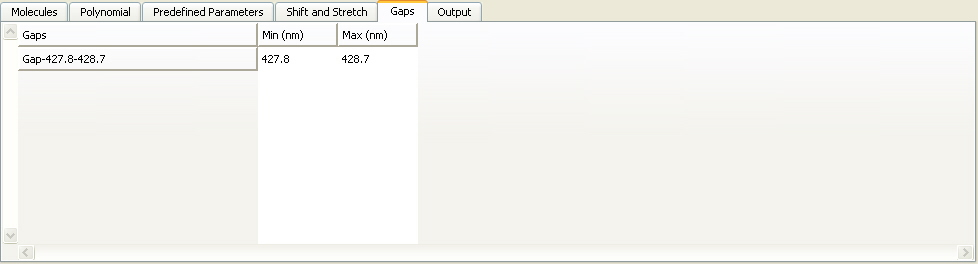
\includegraphics[width=\textwidth]{img/Analysis_Gaps.jpg}
\caption{Analysis Windows Properties: Gaps Page}\label{analysis_gaps}
\end{figure}
\FloatBarrier

\subsubsection{Insert a gap}
To insert a gap, right-click the \textbf{Insert} option and complete the \textbf{Min (nm)} and \textbf{Max (nm)} columns with the limits given in nanometers.  The first column is automatically updated after validation of the entry fields.

\subsubsection{Remove a gap}
To remove a gap, select it in the \textbf{Gaps} column and right-click the \textbf{Remove} option.

\subsection{The Output Pages}
For each cross section defined in the \textbf{Molecules} page, this page proposes to select the analysis results to save in the ASCII output file(s). Columns are enabled only if the \textbf{Analysis} button is checked in the \textbf{Output page} of \textbf{Projects properties}.

\begin{figure}[!h]
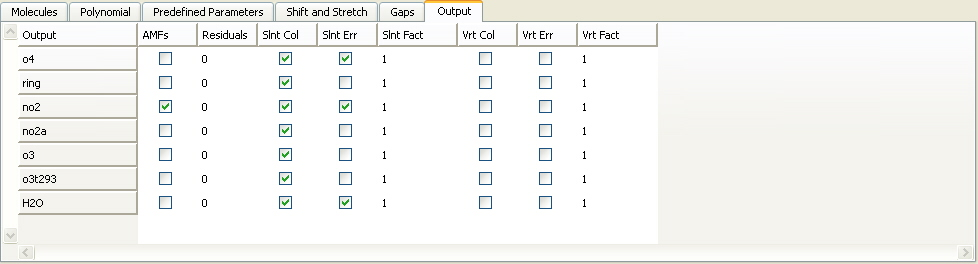
\includegraphics[width=\textwidth]{img/Analysis_Output.jpg}
\caption{Analysis Windows Properties: Output Page}\label{analysis_output}
\end{figure}
\FloatBarrier

QDOAS calculates and saves vertical columns if an \gls{amf} dependency has been selected in the \textbf{Molecules} page. The \textbf{Residuals} column gives the possibility to specify a value for the residual column amount of the selected species in the reference spectrum.

In the output file, slant columns and vertical columns (and their respective errors) can be divided by a scaling factor using \textbf{Slnt Fact} and \textbf{Vrt Fact} edit controls.

In the output file, the title of columns with the retrieval results always starts with the name of the analysis window. Slant columns are indicated by \textbf{SlCol}, standard deviations by \textbf{SlErr}, vertical columns by \textbf{VCol}, air mass factors \textbf{AMF}, etc\dots For example, if the application contains two analysis windows (no2 and o3), no2.slcol(o3) and o3.slcol(no2) refer to the column titles for respectively the slant columns of O3 in the no2 window and NO2 in the o3 fitting window.

Examples of output generated by QDOAS can be found in appendix \textbf{~\ref{cha:output}}.

\section{Configuration of the wavelength calibration procedure}\label{sec:conf-wavel-calibr}
The wavelength calibration facility developed in QDOAS is based on a
\gls{nlls} fitting procedure where the shift between the spectrum we
want to calibrate and a highly accurate solar reference spectrum is
determined on a series of short wavelength intervals.  The fitting
procedure uses the same algorithms used for the analysis of
spectra. The \textbf{Analysis Method} (optical density fitting or
intensity fitting) can be different from the one selected for the
analysis of spectra in the \textbf{Analysis page}.

The calibration procedure also allows the characterisation of the
instrumental slit function, through fitting of user-defined
\glspl{sfp}, either the \gls{fwhm} of an analytical line shape (see
the \textbf{\nameref{sec:analyt-line-shap}}, page
\pageref{sec:analyt-line-shap}) or two different stretch factors
applied on the grid of a user-defined function (option \textbf{File}).
If the slit function is not fitted during the wavelength calibration
procedure, the solar spectrum and the instrumental line shape to use
for convolutions are defined in the \textbf{Slit page}, page
\pageref{sec:projects_slit_page}.

The wavelength calibration can be applied to any kind of spectrum (the
reference spectra or spectra to analyze).

The wavelength calibration can be configured in the
\textbf{Calibration} page of the project properties.  We explain the
different settings below.

\begin{figure}[!h]
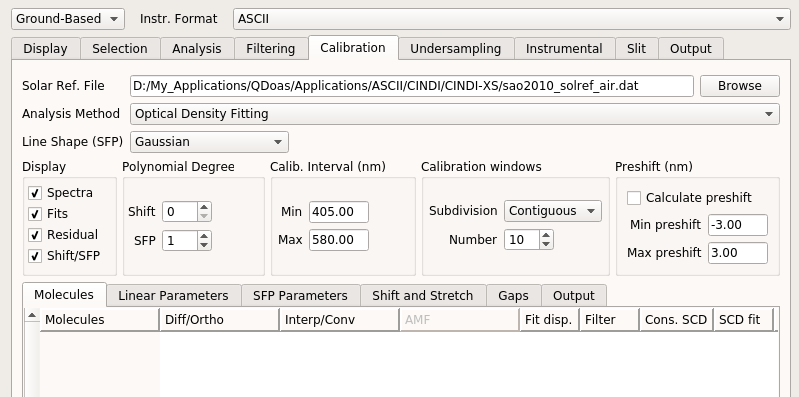
\includegraphics[width=\textwidth]{img/Project_Calibration.png}
\caption{Projects properties: Calibration page}\label{projects_properties_calibration}
\end{figure}
\FloatBarrier

\subsection{Solar Reference File and Line Shape}
There are two cases to consider:
\begin{enumerate}
\item The slit function (line shape) of the instrument is known and
  there is no need to characterise it once again (\textbf{Line Shape}
  ``Don't fit'').  Then the \textbf{Solar Ref. File} in this page is
  disabled; it should be given in the \textbf{Slit page}, together
  with the known instrumental line shape.
\item The slit function of the instrument needs to be characterized
  (selection of a \textbf{Line Shape}): the \textbf{Solar Ref. File}
  should contain a high-resolution solar spectrum.  Because the
  convolution algorithm in QDOAS uses the Fourier transform to speed
  up the \gls{nlls} fitting, a high-resolution solar spectrum sampled
  on a constant grid is expected.
\end{enumerate}

\subsection{Display}
When the calibration procedure is applied, a page named ``Kurucz''
appears in the plot area of the program except if the
\textbf{Calibration fits} button is unchecked in the \textbf{Display
  page}. This page includes four kinds of plots:

\begin{description}
\item[Spectra] the complete fit between the observed and the calculated spectra;
\item[Fits] fit of the Ring effect and/or atmospheric absorptions if any;
\item[Residual] the residual of the fit;
\item[Shift/SFP] the wavelength dependency of the shift and the slit function parameters over the whole detector.
\end{description}

\subsection{Polynomial Degree}
When the fitting procedure for each subwindow has finished, a
polynomial is used to approximate the shift values determined in each
subwindow.  This polynomial is then used to correct the initial
wavelength calibration.  Similarly, the wavelength dependent slit
function is determined by fitting a polynomial through the individual
SFP values. A different \textbf{polynomial degree} can be specified
for the shift and for the slit function.  The wavelength calibration
and the variation of the slit function thus determined are then used
e.g.\ to convolve high resolution cross sections before the analysis
of spectra and to build undersampling cross sections.

\subsection{Calibration Interval}
The wavelength interval used for the calibration must be specified in
the \textbf{Calib.\ Interval (nm)} frame. It should cover all the
spectral analysis windows defined under the \textbf{Analysis Windows}
node of the projects tree. This calibration interval is divided in a
number of \textbf{subwindows} and the shift and the \glspl{sfp} are
fitted using the \gls{nlls} approach within each of these subwindows.
The settings in the frame \textbf{Calibration windows} control the
definition of these subwindows.

\subsection{Calibration Windows}\label{sec:calibration-windows}
During the calibration procedure, the calibration interval is divided
into a number of smaller intervals.  The settings in the \textbf{Calibration
Windows} frame can be used to define these intervals.  The user can
set the number of intervals to be used, and set their limits using one
of the following options from the \textbf{Subdivision} drop-down menu:

\begin{description}
\item[Contiguous] With the default ``Contiguous'' option, the complete
  calibration interval is divided into non-overlapping subwindows of
  equal size.
\item[Sliding] The more general ``Sliding'' option allows the user to
  choose the width of the subwindows (``Size (nm)''), independently
  from the number of subwindows.  The calibration interval is now
  divided into a number of equally spaced subwindows, which can be
  made to overlap by choosing a larger size, or made disjoint by
  choosing a smaller size.  Usually, one wants to increase the size of
  the subwindows in order to improve the stability of the calibration
  fit in each subwindow.
\item[Custom] With the ``Custom'' option, the user can manually set
  the limits of the subintervals used in the calibration.  Clicking on
  the ``Define windows'' button opens a pop-up where the lower and
  upper wavelength limit can be configured for each subwindow.
\end{description}

\subsection{Fitting Parameters}
The wavelength calibration uses a similar property sheet as the
\nameref{analysis_properties} to configure the fitting procedure for
the calibration subwindows.  The configuration of these pages is
usually limited to the specification of the degree of the polynomial
uses in the DOAS equation (different from the polynomial used to build
the final grid from the individual values of the shift resulting from
the fit as described above), the slit function parameters to fit
according to the selection of the line shape and the shift between the
spectrum to calibrate and the solar spectrum. But the algorithm can
also take into account atmospheric absorption, Ring effect and offset
correction.

\subsubsection{The Molecules page}
The \textbf{Molecules} page allows introducing correcting absorbers that may optimise the accuracy of the wavelength calibration, e.g. the Ring effect (when calibrating a scattered-light spectrum) and \ozone~absorption can be taken into account in the fit.

\begin{figure}[!h]
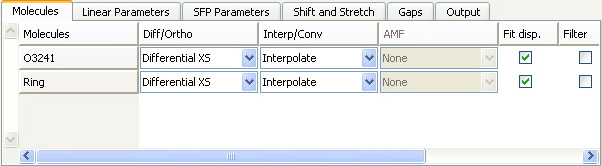
\includegraphics[width=.8\textwidth]{img/Calibration_Molecules.jpg}\hfill

\vspace{6pt}

\hfill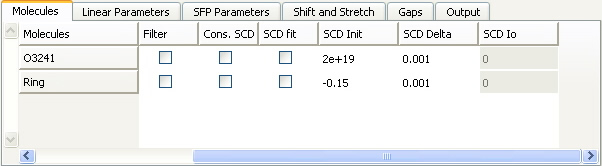
\includegraphics[width=.8\linewidth]{img/Calibration_Molecules2.jpg}
\caption{Calibration Properties: Molecules Page}\label{calibration_molecules}
\end{figure}

To generate differential cross sections (column \textbf{Diff/Orthog}), see page \pageref{differential_xs}.  The \textbf{Fit display} column is activated only if the \textbf{Calibration} button is checked in the \textbf{Display} page of \textbf{Projects properties} (see page \pageref{sec:projects_display_page}) and if the \textbf{Fits} button is checked in the \textbf{Display} frame of the \textbf{Calibration} page (see page \pageref{sec:projects_calibration_page}).  The selected cross section are usually pre-convolved with the resolution of the instrument and interpolated on the grid of the control (reference) spectrum.

In order to optimise the accuracy of the calibration (and given limitations inherent to the method), it is recommended to limit the number of parameters to fit and to constrain the slant column density of molecules.  This can be done in two passes:

\begin{itemize}
\item in the first pass, the column density is fitted (\textbf{SCD Fit} button is checked) over the whole calibration interval; a mean value of the concentration is then determined from the sub intervals where the fitting of the cross section has a sense (where the spectral information is largest);
\item in the second pass, the concentration is fixed at the mean value determined at the previous pass.
\end{itemize}

See previous section (\ref{sec:analysis_config_param}) for a complete description of the columns in this page.

\subsubsection{The Linear Parameters Page}
In this page, you define the polynomial used to approximate the
continuous component of the spectrum to calibrate.  To generate
differential cross sections using the orthogonalisation method, don't
forget to build an orthogonal base (see page
\pageref{differential_xs}).

\subsubsection{The Slit Function Parameters Page}
The fit of the \glspl{sfp} can be configured in this page.  There are
two predefined parameters -- SFP 1 and SFP 2 -- whose role depends on
the line shape chosen in the \textbf{Line Shape (SFP)} drop-down menu.
Note that if you do not want to fit the slit function during the wavelength
calibration procedure, select \textbf{Don't fit} in the Line Shape
menu and choose a solar reference spectrum and line shape in the
\textbf{Slit Page} of \textbf{Projects properties} (see page
\pageref{sec:projects_slit_page}) instead.

\begin{figure}[!h]
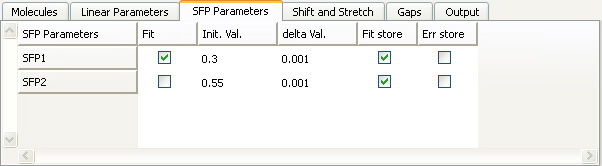
\includegraphics[width=\textwidth]{img/Calibration_Predefined2.jpg}
\caption{Calibration Properties: SFP Parameters Page (Parameterisation for an error function line shape)}\label{calibration_sfp}
\end{figure}

Table \ref{tab:sfp_meanings} provides an overview of the meaning of
SFP 1 and 2 for the different possible line shapes.  For analytical
line shapes, \textbf{SFP 1} is generally used for fitting the
\gls{fwhm} of the selected line shape.  The Voigt profile function is
the convolution of a Gaussian and a Lorentzian line shapes, where the
second parameter is the Lorentz/Gauss ratio.  Asymmetric line shapes
can be fitted by introducing an asymmetry factor in the Gaussian
formula.  For two-parameter line shapes, it is generally recommended
to fix one of the parameters to an estimated value in order to avoid
numerical instabilities.

\begin{table}\label{tab:sfp_meanings}
  \centering
  \setlength\tabcolsep{3.5pt} % default value: 6pt
  \begin{longtable}{lcc}
    \toprule
    & \textbf{SFP 1} & \textbf{SFP 2} \\
    \midrule
    \textbf{File}	& Stretch factor & Stretch factor \\
    & (negative wavelengths)	& (positive wavelengths)	\\
    \textbf{Gaussian}	& \gls{fwhm}	& Ignored \\
    \textbf{Error function}	& FWHM	& Boxcar width \\
    \textbf{2n-Lorentz}	& FWHM	& Ignored \\
    \textbf{Voigt profile}	& FWHM (Gaussian)	& Lorentz/Gauss ratio \\
    \textbf{Asymmetric Gaussian}	& FWHM (Gaussian)	& Asymmetry factor \\
    \bottomrule
  \end{longtable}
\caption{Meaning of the SFP parameters for different types of line
shape.}
\end{table}

\subsubsection{The Shift and Stretch Pages}
For the configuration of these pages, refer to the previous section (\ref{sec:shift_stretch_page}, page \pageref{sec:shift_stretch_page}).  In order to avoid the interpolation of the spectrum to calibrate, it is recommended to fit the shift of the high-resolution solar spectrum, represented by the symbol \textbf{Ref}.

\textit{In this case, all cross sections defined in the \textbf{Molecules} page have to be shifted with the solar spectrum.}

\begin{figure}[!h]
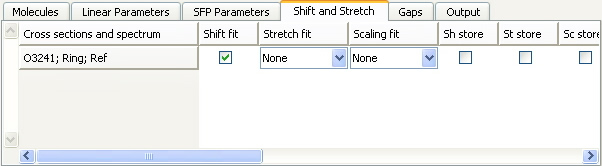
\includegraphics[width=\textwidth]{img/Calibration_Shift.jpg}
\caption{Calibration Properties: Shift Page (The \ozone~and Ring cross sections defined in the \textbf{Molecules} page are shifted with the solar spectrum.)}\label{calibration_shift}
\end{figure}

\subsubsection{Output}
Fitted slant column densities and non linear parameters are saved in the output file if the \textbf{``Calibration''} button is checked in \textbf{Output Page} of \textbf{Projects properties}.  This is particularly useful if a \textbf{Run Calibration} is performed on all spectra of the file.

\subsection{Calculation of the preshift} \label{sec:projects_calibration_preshift}
If the wavelength calibration of the reference spectrum is really too bad, the calibration procedure couldn't converge and return a wrong value of the shift that corresponds to a local minimum of the chi square.  In this case, it could be useful to approximate the value of the shift by calculating the
correlation between the reference spectrum and the solar spectrum convolved at the resolution of the instrument using the initial value(s) of the slit function parameter(s).  The value of the shift giving the best correlation will be introduced by the program as initial shift of the usual NLLS algorithm.
To calculate the preshift before the Kurucz procedure, check the \textbf{``Calculate preshift''} button in the \textbf{``Preshift (nm)''} frame and define the interval in nanometers wherein the shift values can vary for the correlation test.

%%% Local Variables:
%%% mode: latex
%%% TeX-master: "QDOAS_manual"
%%% TeX-PDF-mode: t
%%% End:
